\SSbreak\\
\emph{Source: \Cop}\\
\emph{Proposer: \Phobo}\\ %\Pchan \Pbrain \Pss
\emph{Problem ID: 142}\\
\emph{Date: 2021-02-24}\\
\emph{Difficulty: Easy}\\
\SSbreak

\SSpsetQ{
	In the following diagram every circle has two internally tangent circles also tangent to each other. The radius of the biggest circle is $\frac{1}{\sqrt{\pi}}$. If the area of the black region can be expressed as $\frac{a}{b}$, compute $100a+b$.
	%Put Problem Here
}\bigskip

\begin{figure}[ht]
	\centering
	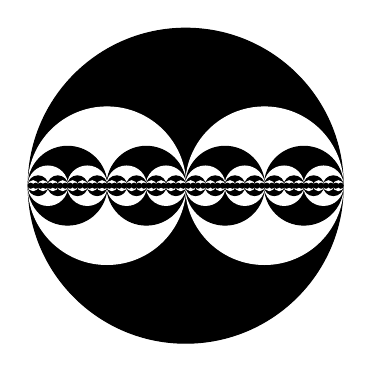
\begin{tikzpicture}
		\foreach \x in {0}  \draw[fill,color = black] (\x,0) circle (2cm);
		\foreach \x in {0,...,1}  \draw[fill,color = white] (-1+2*\x,0) circle (1cm);
		\foreach \x in {0,...,3}  \draw[fill,color = black] (-1.5+1*\x,0) circle (0.5cm);
		\foreach \x in {0,...,7}  \draw[fill,color = white] (-1.75+0.5*\x,0) circle (0.25cm);
		\foreach \x in {0,...,15} \draw[fill,color = black] (-1.875+0.25*\x,0) circle (0.125cm);
		\foreach \x in {0,...,31} \draw[fill,color = white] (-1.9375+0.125*\x,0) circle (0.0625cm);
		\foreach \x in {0,...,63} \draw[fill,color = black] (-1.96875+0.0625*\x,0) circle (0.03125cm);
	\end{tikzpicture}
\end{figure}

\begin{solution}[Solution by \Phobo]\hfil\medskip
	
	Let $r_n$ and $A_n$ be the radius and the area of the nth circle (in descending order). From construction we have $r_{n+1}=\frac{r_{n}}{2}$ which leads to $r_n=\frac{r_0}{2^n}$, where $r_0=\frac{1}{\sqrt{\pi}}$. Looking at the desired area $A_{\zeta}$ as difference of black and white circles areas, we get the following:
	\begin{align}
		A_{\zeta}&= \sum_{n=0}^{\infty}(-2)^n A_{n} \\
		&=\sum_{n=0}^{\infty}(-2)^n (r_n)^2 \pi \\
		&=(r_0)^2 \pi \sum_{n=0}^{\infty}\left(-\frac{1}{2}\right)^n \\
		&=\left(\frac{1}{\sqrt{\pi}}\right)^2\pi\frac{1}{1-\left(-\frac{1}{2}\right)} \\ 
		&= \frac{2}{3}
	\end{align}
	Which means $\boxed{203}$ is the solution.
\end{solution}\bigskip

\begin{solution}[Solution by \Pflame]\hfil\medskip

	Let $B$ be the total black area; the total white area is then $1 - B$. Looking at the two biggest white circles, we see that each of them is similar
	to the big circle by a factor of $\frac{1}{2}$ with colors inverted; thus the total black area inside each of the two white circles is $\frac{1 - B}{4}$.
	Since the black area outside the two big white circles is $\frac{1}{2}$ we have $$B = \dfrac{1}{2} + \dfrac{1 - B}{2} \iff B = \dfrac{2}{3} \iff \boxed{203}.$$
\end{solution}